%!TEX TS-program = xelatex
\documentclass[notes,12pt, aspectratio=169]{beamer}

\usepackage{amsmath,amsfonts,amssymb,amsthm,mathtools}  % пакеты для математики
\usepackage{minted}

\usepackage[english, russian]{babel} % выбор языка для документа
\usepackage[utf8]{inputenc} % задание utf8 кодировки исходного tex файла
\usepackage[X2,T2A]{fontenc}        % кодировка

\usepackage{fontspec}         % пакет для подгрузки шрифтов
\setmainfont{Helvetica}  % задаёт основной шрифт документа

% why do we need \newfontfamily:
% http://tex.stackexchange.com/questions/91507/
\newfontfamily{\cyrillicfonttt}{Helvetica}
\newfontfamily{\cyrillicfont}{Helvetica}
\newfontfamily{\cyrillicfontsf}{Helvetica}

\usepackage{unicode-math}     % пакет для установки математического шрифта
% \setmathfont{Neo Euler} % шрифт для математики

\usepackage{polyglossia}      % Пакет, который позволяет подгружать русские буквы
\setdefaultlanguage{russian}  % Основной язык документа
\setotherlanguage{english}    % Второстепенный язык документа

% Шрифт для кода
\setmonofont[Scale=0.85]{Monaco}
\usepackage{verbments}

\usepackage{pgfpages}
% These slides also contain speaker notes. You can print just the slides,
% just the notes, or both, depending on the setting below. Comment out the want
% you want.
%\setbeameroption{hide notes} % Only slide
%\setbeameroption{show only notes} % Only notes
%\setbeameroption{show notes on second screen=right} % Both

\usepackage{array}

\usepackage{tikz}
\usepackage{verbatim}
\setbeamertemplate{note page}{\pagecolor{yellow!5}\insertnote}
\usetikzlibrary{positioning}
\usetikzlibrary{snakes}
\usetikzlibrary{calc}
\usetikzlibrary{arrows}
\usetikzlibrary{decorations.markings}
\usetikzlibrary{shapes.misc}
\usetikzlibrary{matrix,shapes,arrows,fit,tikzmark}

\usepackage{hyperref}
\usepackage{lipsum}
\usepackage{multimedia}
\usepackage{multirow}
\usepackage{dcolumn}
\usepackage{bbm}
\newcolumntype{d}[0]{D{.}{.}{5}}

\usepackage{changepage}
\usepackage{appendixnumberbeamer}
\newcommand{\beginbackup}{
   \newcounter{framenumbervorappendix}
   \setcounter{framenumbervorappendix}{\value{framenumber}}
   \setbeamertemplate{footline}
   {
     \leavevmode%
     \hline
     box{%
       \begin{beamercolorbox}[wd=\paperwidth,ht=2.25ex,dp=1ex,right]{footlinecolor}%
%         \insertframenumber  \hspace*{2ex} 
       \end{beamercolorbox}}%
     \vskip0pt%
   }
 }
\newcommand{\backupend}{
   \addtocounter{framenumbervorappendix}{-\value{framenumber}}
   \addtocounter{framenumber}{\value{framenumbervorappendix}} 
}

% для имитации питоновского синтаксиса 
\newcommand{\pgr}[1]{{\color{green} \textbf{#1}}}


%%%%%%%%%% Работа с картинками %%%%%%%%%
\usepackage{graphicx}                  % Для вставки рисунков
\usepackage{graphics}
\graphicspath{{images_2/}}    % можно указать папки с картинками
\usepackage{wrapfig}                   % Обтекание рисунков и таблиц текстом

\usepackage[space]{grffile}
\usepackage{booktabs}

% These are my colors -- there are many like them, but these ones are mine.
\definecolor{blue}{RGB}{0,114,178}
\definecolor{red}{RGB}{213,94,0}
\definecolor{yellow}{RGB}{240,228,66}
\definecolor{green}{RGB}{0,128, 0}

\hypersetup{
  colorlinks=false,
  linkbordercolor = {white},
  linkcolor = {blue}
}


%% I use a beige off white for my background
\definecolor{MyBackground}{RGB}{255,253,218}

%% Uncomment this if you want to change the background color to something else
%\setbeamercolor{background canvas}{bg=MyBackground}

%% Change the bg color to adjust your transition slide background color!
\newenvironment{transitionframe}{
  \setbeamercolor{background canvas}{bg=yellow}
  \begin{frame}}{
    \end{frame}
}

\setbeamercolor{frametitle}{fg=blue}
\setbeamercolor{title}{fg=black}
\setbeamertemplate{footline}[frame number]
\setbeamertemplate{navigation symbols}{} 
\setbeamertemplate{itemize items}{-}
\setbeamercolor{itemize item}{fg=blue}
\setbeamercolor{itemize subitem}{fg=blue}
\setbeamercolor{enumerate item}{fg=blue}
\setbeamercolor{enumerate subitem}{fg=blue}
\setbeamercolor{button}{bg=MyBackground,fg=blue,}


% If you like road maps, rather than having clutter at the top, have a roadmap show up at the end of each section 
% (and after your introduction)
% Uncomment this is if you want the roadmap!
% \AtBeginSection[]
% {
%    \begin{frame}
%        \frametitle{Roadmap of Talk}
%        \tableofcontents[currentsection]
%    \end{frame}
% }
\setbeamercolor{section in toc}{fg=blue}
\setbeamercolor{subsection in toc}{fg=red}
\setbeamersize{text margin left=1em,text margin right=1em} 

% списки, которые растягиваются на всю величину слайда 
\newenvironment{wideitemize}{\itemize\addtolength{\itemsep}{10pt}}{\enditemize}



\title[]{\textcolor{blue}{Практический анализ данных и машинное обучение: искусственные нейронные сети}}
\author{Ульянкин Филипп}
\date{\today}


\begin{document}

%%% TIKZ STUFF
\tikzset{   
        every picture/.style={remember picture,baseline},
        every node/.style={anchor=base,align=center,outer sep=1.5pt},
        every path/.style={thick},
        }
\newcommand\marktopleft[1]{%
    \tikz[overlay,remember picture] 
        \node (marker-#1-a) at (-.3em,.3em) {};%
}
\newcommand\markbottomright[2]{%
    \tikz[overlay,remember picture] 
        \node (marker-#1-b) at (0em,0em) {};%
}
\tikzstyle{every picture}+=[remember picture] 
\tikzstyle{mybox} =[draw=black, very thick, rectangle, inner sep=10pt, inner ysep=20pt]
\tikzstyle{fancytitle} =[draw=black,fill=red, text=white]
%%%% END TIKZ STUFF

% Title Slide
\begin{frame}
\maketitle
\centering Автокодировщики, трюки, используемые при обучении сеток
\end{frame}


\begin{frame}{Agenda} 
\begin{wideitemize}
	\item Автокодировщики
	
	\item Эвристики, используемые при обучении нейронных сетей 
\end{wideitemize}
\end{frame}


\begin{transitionframe}
	\begin{center}
		\Huge  Автокодировщики 
	\end{center}
\end{transitionframe}


\begin{frame}{Автокодировщики}
\begin{wideitemize}
	\item Понижение размерности --- задача обучения без учителя
	\item Давайте превратим её в обучение с учителем! 
\end{wideitemize}
\end{frame}


\begin{frame}{Автокодировщики}
\begin{center}
		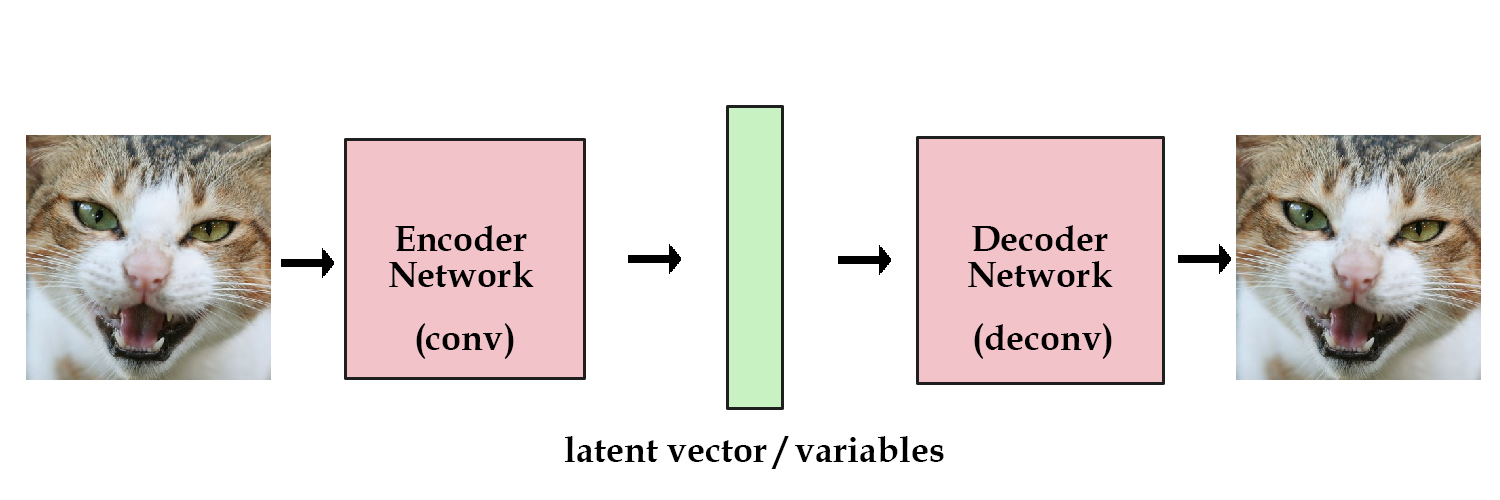
\includegraphics[width=.9\linewidth]{autoencoder.png}
\end{center}
\end{frame}


\begin{transitionframe}
	\begin{center}
		\Huge Собираем свой автокодировщик
	\end{center}
\end{transitionframe}


\begin{transitionframe}
	\begin{center}
		\Huge  Эвристики для обучения сеток 
	\end{center}
\end{transitionframe}


\begin{frame}{Эвристики, используемые при обучении}
\begin{wideitemize}
	\item Применимы все те же эвристики, что и в градиентном спуске 
	
	\item Инициализация весов, выбор шага, порядок предъявления объектов
	
	\item Кроме того появляются новые проблемы: выбор функции активации в каждом нейроне, выбор числа слоёв, числа нейронов, выбор значимых связей
	
	\item Это приводит к возникновению новых эвристик 
\end{wideitemize}
\end{frame}


\begin{transitionframe}
	\begin{center}
		\Huge  Функции активации
	\end{center}
\end{transitionframe}




\begin{frame}{Sigmoid activation}
\begin{center}
	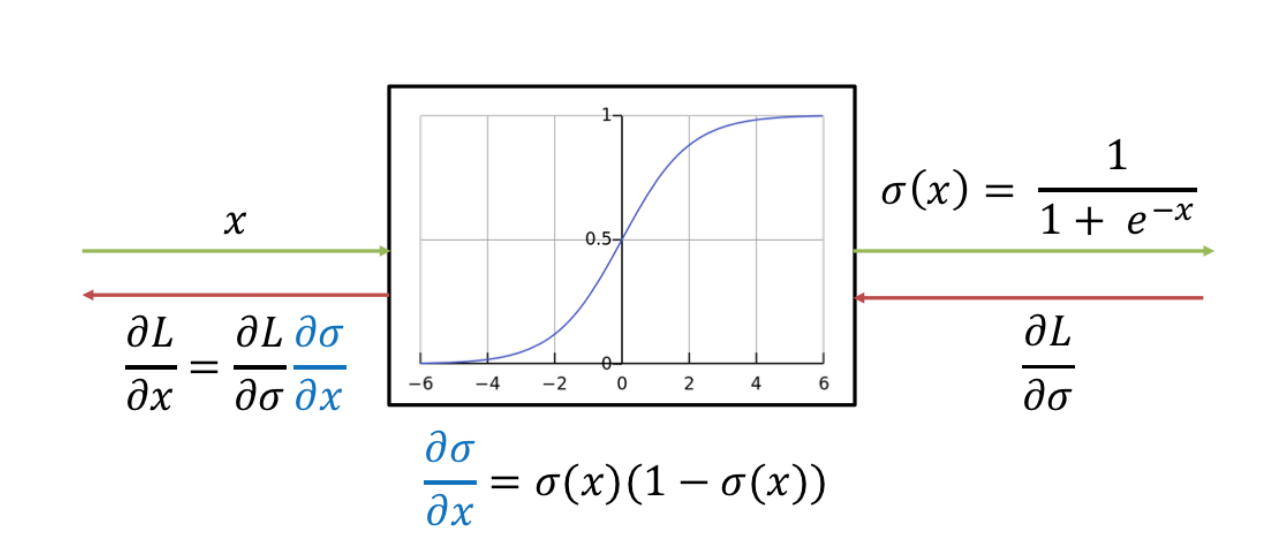
\includegraphics[width=.8\linewidth]{sigmoid_activation.png}
\end{center}


\begin{itemize}
{\color{red} 
	\item В глубоких сетях способствует затуханию градиента (vanishing gradients)
	
	\item Не центрирована относительно нуля
	
	\item Вычислять $e^x$ дорого
}
\end{itemize}

\end{frame}


\begin{frame}{Tanh activation}
\begin{center}
	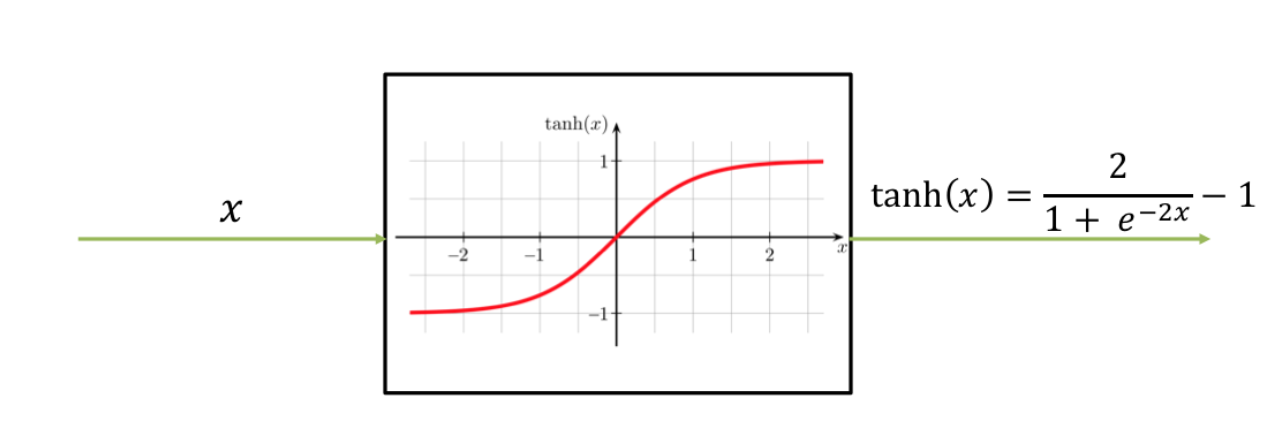
\includegraphics[width=.8\linewidth]{tanh_activation.png}
\end{center}

\begin{itemize}
	\item  {\color{green}  Центрирован относительно нуля }
	
	\item  {\color{red}  Всё ещё похож на сигмоиду }
	
\end{itemize}
\end{frame}


\begin{frame}{ReLU activation}
\begin{center}
	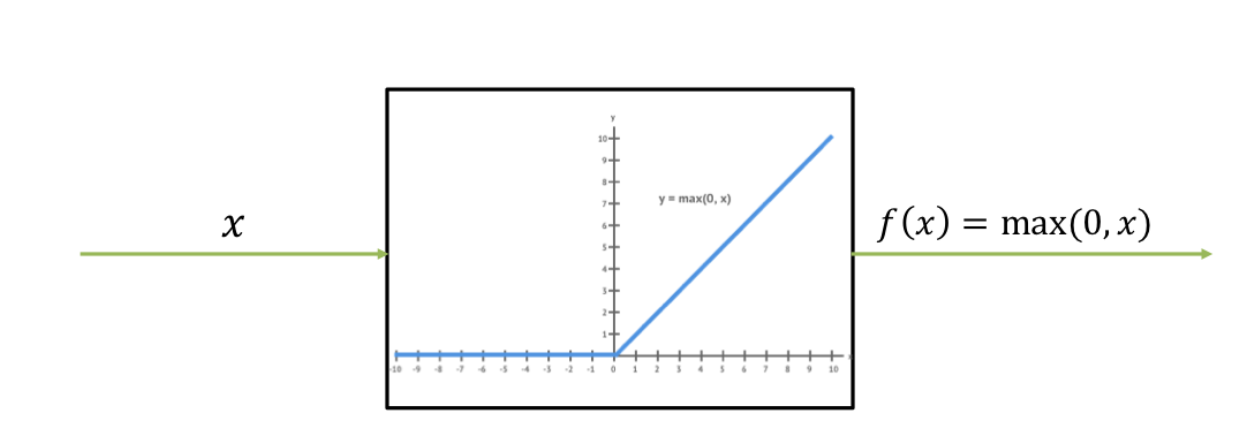
\includegraphics[width=.8\linewidth]{relu_activation.png}
\end{center}

\begin{itemize}
	{ \color{green} 
		\item  Быстро вычисляется 
		
		\item  Градиент никогда не зануляется при $x > 0$
		
		\item  Сходимость сеток ускоряется 
	} 
\end{itemize}
\end{frame}


\begin{frame}{ReLU activation}
\begin{center}
	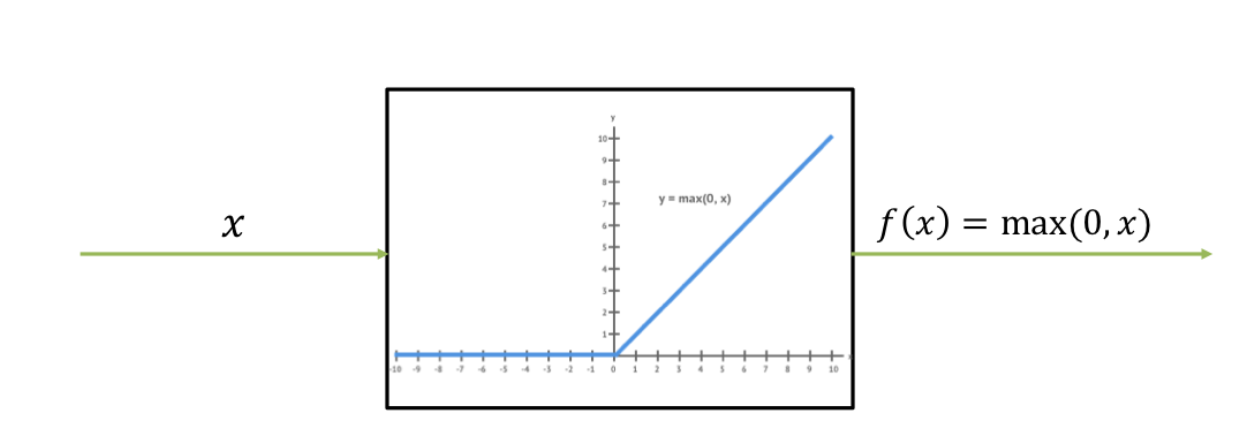
\includegraphics[width=.8\linewidth]{relu_activation.png}
\end{center}

\begin{itemize}
	{ \color{red} 
		\item  Сетка может умереть, если активация занулится на всех нейронах
		
		\item  Не центрирован относительно нуля
	} 
\end{itemize}
\end{frame}


\begin{frame}{Leaky ReLU activation}
\begin{center}
	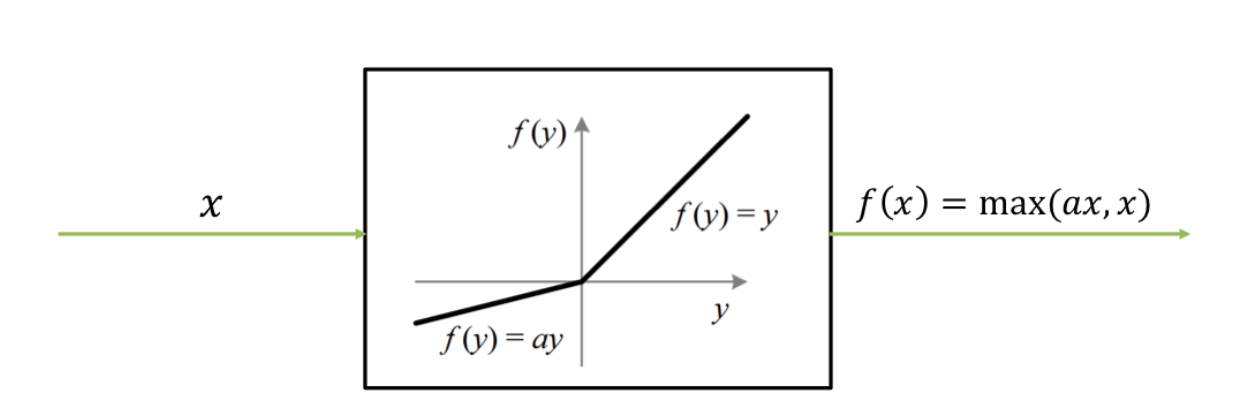
\includegraphics[width=.7\linewidth]{leaky_relu_activation.png}
\end{center}

\begin{itemize}
	{ \color{green} 
	\item  Как ReLU, но не умирает
	\item Важно, чтобы $a \ne 1$
} 
\end{itemize}
\end{frame}


\begin{frame}{Что же выбрать}
\begin{wideitemize}
	\item  На самом деле это неважно
	
	\item Важно собрать хорошую архитектуру и подобрать метод оптимизации
	
	\item Обычно в сетках работают либо с сигмоидом либо с ReLU, если остаётся время, то пробуют другие идеи, но обычно выгрыш в качестве от перебора в функциях активации довольно низкий
\end{wideitemize}
\end{frame}



\begin{transitionframe}
	\begin{center}
		\Huge  Дропаут 
	\end{center}
\end{transitionframe}


\begin{frame}{Dropout}
\begin{wideitemize}
	\item Придумали в 2014 году
	
	\item С вероятностью $p$ отключаем нейрон 
	
	\item Делает нейроны более устойчивыми к случайным возмущениям
	
\end{wideitemize}

\begin{center}
	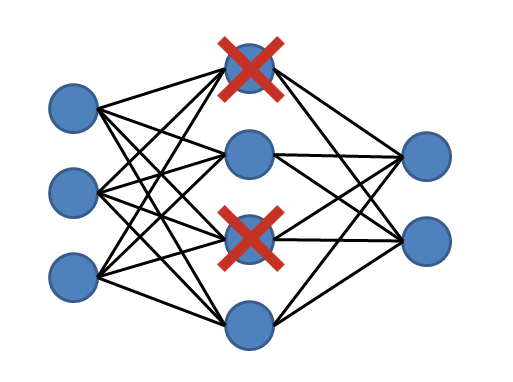
\includegraphics[width=.4\linewidth]{dropout.png}
\end{center}
\end{frame}


\begin{frame}{Dropout}
\begin{wideitemize}
	\item  На каждой итерации мы изменяем только часть параметров, обучение нейронов протекает чуть более независимо
	
	\item При тестировании все нейроны присутствуют в сетке, но их выходы домножаются на вероятность $p$ 
	
	\item На самом деле с байесовской точки зрения, вводя дропаут, мы обучаем ансамбль нейронных сетей
\end{wideitemize}
\end{frame}


\begin{transitionframe}
	\begin{center}
		\Huge  Регуляризация
	\end{center}
\end{transitionframe}


\begin{frame}{Регуляризация}
\begin{wideitemize}
	\item $L_2$: приплюсовываем к функции потерь $\lambda \cdot \sum w_i^2$
	
	\item $L_1$: приплюсовываем к функции потерь $\lambda \cdot \sum |w_i|$
	
	\item Можно регуляризовать не всю сетку, а отдельный нейрон или слой 
	
	\item Не даёт нейрону сфокусироваться на слишком выделяющемся входе
	
	\item Очень похожа по своему действию на droput
\end{wideitemize}
\end{frame}


\begin{transitionframe}
	\begin{center}
		\Huge  Early stopping
	\end{center}
\end{transitionframe}


\begin{frame}{Early stopping}
\begin{wideitemize}
	\item Подбор числа шагов для обучения на основе провреки на валидации
	
	\item Для линейной модели с квадратичной (MSE) функцией потерь и SGD рання остановка эквивалентна $L_2$ регуляризации 
\end{wideitemize}

\begin{center}
	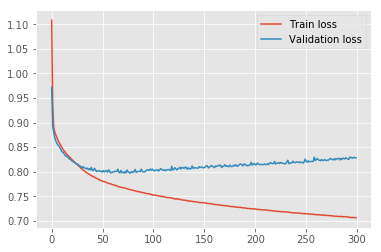
\includegraphics[width=.5\linewidth]{early_stopping.png}
\end{center}
\end{frame}



\begin{transitionframe}
	\begin{center}
		\Huge  Batchnorm
	\end{center}
\end{transitionframe}


\begin{frame}{Стандартизация}
\begin{center}
	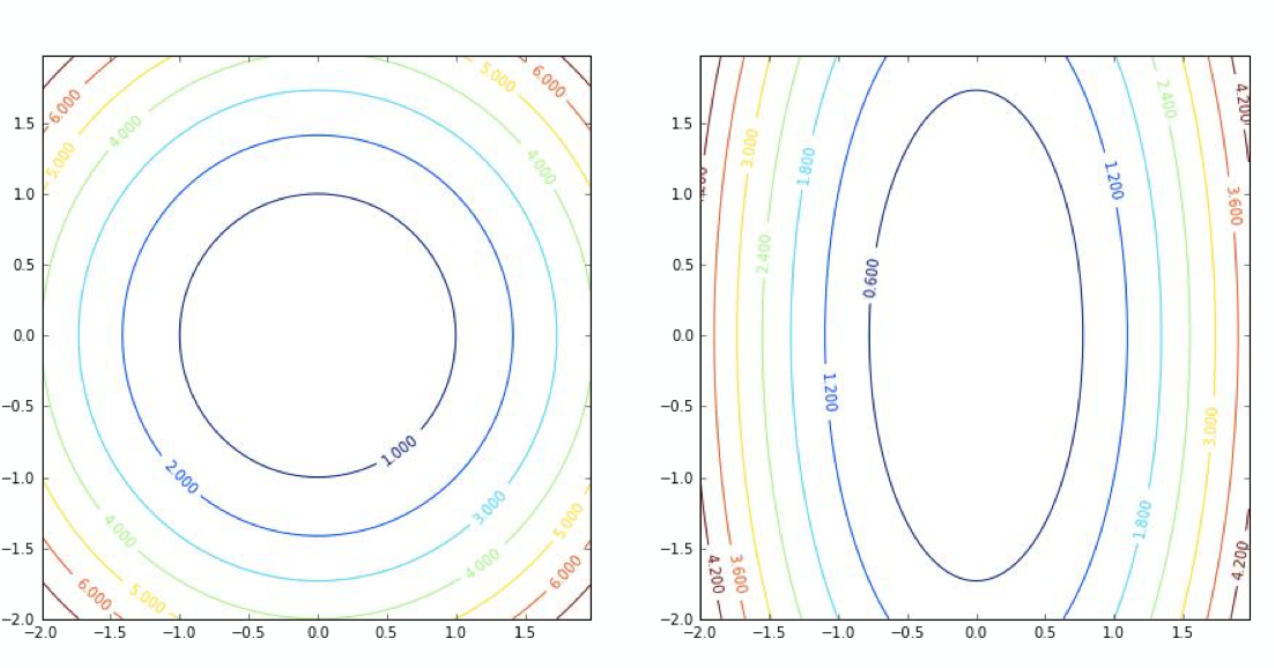
\includegraphics[width=.8\linewidth]{standartization.png}
\end{center}

\begin{center}
 Какая из ситуаций лучше для SGD? 
\end{center}
\end{frame}


\begin{frame}{Batch norm}
\begin{wideitemize}
	\item Придумали в 2015 году 
	\item Давайте вместо $X$ на входе использовать $\frac{X - \mu_X}{\sigma_X}$
	\item Давайте на каждом слое вместо $f(XW)$ использовать  $\frac{f(XW) - \mu_f}{\sigma_f}$
	\item Обучение довольно сильно ускоряется 
\end{wideitemize}
\end{frame}


\begin{transitionframe}
	\begin{center}
		\Huge Инициализация модели
	\end{center}
\end{transitionframe}


\begin{frame}{Инициализация весов}
\begin{wideitemize}
	\item Наши признаки $X$ пришли к нам из какого-то распределения 
	\item Выход слоя $f(XW)$ будет принадлежать другому распределению 
	\item Если инициализировать веса неправильно, дисперсия распределения може от слоя к слою увеличиваться
	\item Эмпирически было выяснено, что это может портить сходимость для глубоких сеток 
\end{wideitemize}
\end{frame}


\begin{frame}{Инициализация весов}
\begin{wideitemize}
	\item  Для симметричных функций с нулевым средним используйте инициализацию Ксавье {\color{green}  init="glorot\_uniform"} или {\color{green} }
	\item  Для ReLU и им подобным инициализацию Хe {\color{green} init="he\_uniform"} или {\color{green} init="he\_nomal"}
	\item  Если в кратце, эти две инициализации корректируют параметры распределений в зависимости от входа и выхода слоя так, чтобы держать дисперсию в узде
\end{wideitemize}
\end{frame}



\begin{transitionframe}
	\begin{center}
		\Huge  Data augmentation
	\end{center}
\end{transitionframe}


\begin{frame}{Data augmentation}
\begin{center}
	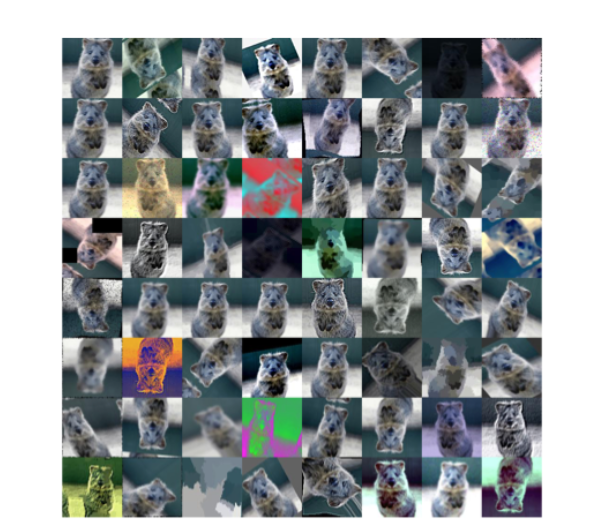
\includegraphics[width=.55\linewidth]{data_augmentation.png}
\end{center}
\end{frame}


\begin{frame}{Data augmentation}
\begin{wideitemize}
	\item  Сдвиги 
	\item Увеличение, уменьшение
	\item Повороты
	\item Искажение
	\item Затенение 
	\item Смена стиля (красок)
\end{wideitemize}

\vfill
\begin{center}
	Делает модель более устойчивой, полезна при маленьких выборках. На больших датасетах также улучшает результаты.
\end{center}
\end{frame}



\begin{transitionframe}
	\begin{center}
		\Huge  Другие приёмы
	\end{center}
\end{transitionframe}

\begin{frame}{Предобучение}
\begin{wideitemize}
\item  Обучаем каждый нейрон на рандомной подвыборке, каждый нейрон впитает какие-то отдельные её особенности, после скрепляем все нейроны вместе и продолжаем обучение на всей выборке

\item  Обучаем на корпусе картинок автокодировщик, encoder благодаря этому учится выделять наиболее важные фичи, которые позволяют эффективно сжимать изображения. После срезаем decoder и на его месте достраиваем слои для решения нашей задаче, запускаем обычное дообучение.
\end{wideitemize}
\end{frame}


\begin{frame}{Динамическое наращивание сети}
\begin{wideitemize}
	\item  Обучение сети при заведомо недостаточном числе нейронов $H$
	\item После стабилизации функции потерь --- добавление нового нейрона и его инициализация путём обучения 
	\begin{itemize}
		\item либо по случайной подвыборке 
		\item либо по объектам с наибольшими значениями потерь 
		\item либо по случайному подмножеству входов
		\item либо из различных случайных начальных приближений
	\end{itemize}
\item Снова итерации BackProp
\end{wideitemize}

\vfill
\begin{center}
\textbf{Эмпирический опыт:} Общее время обучения обычно лишь в $1.5-2$ раза больше, чем если бы в сети сразу было итоговое число нейронов. Полезная информация, накопленная сетью не теряется при добавлении нейронов.
\end{center}
\end{frame}


% сделать этот слайд как у воронцова с кучей формул
\begin{frame}{Прореживание сети}

\begin{wideitemize}
\item Начать с большого количество нейронов и удалять незначимые по какому-нибудь критерию 
\item Пример: обнуляем вес, смотрим как сильно упала ошибка, сортируем все вязи по этому критерию, удаляем $N$ наименее значимых
\item После прореживания снова запускаем backprop
\item Если качество модели сильно упала, вернуть последние удалённые связи 
\end{wideitemize}
\end{frame}


\begin{transitionframe}
	\begin{center}
		\Huge Transfer learning
	\end{center}
\end{transitionframe}

\begin{frame}{Transfer learning}
\begin{wideitemize}
	\item  Глубокие сети извлекают из изображений сложные фичи, но для их обучения нужно много данных...
\end{wideitemize}
	
\begin{center}
	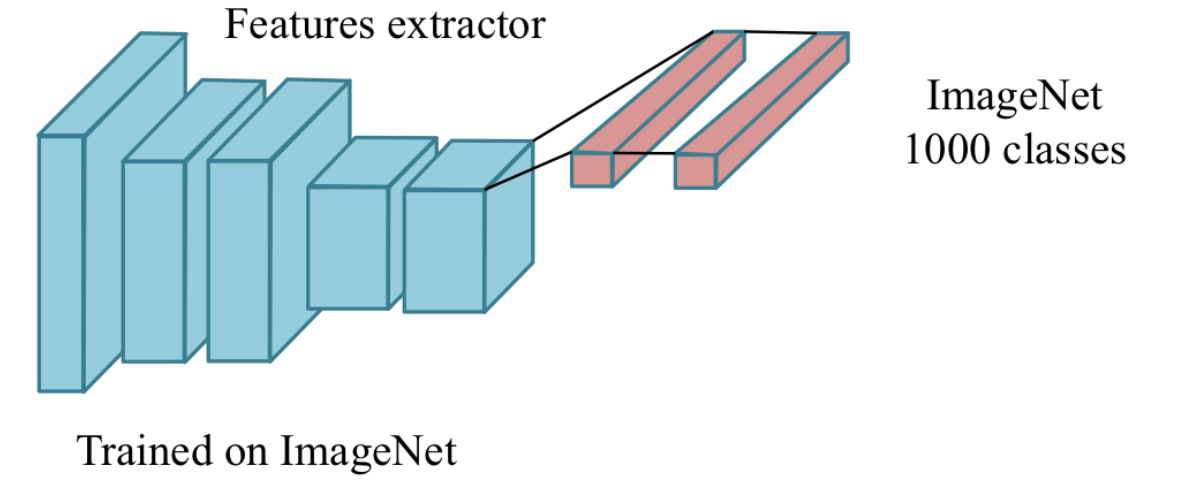
\includegraphics[width=.8\linewidth]{transfer_learning1.png}
\end{center}
\end{frame}

\begin{frame}{Transfer learning}
\begin{wideitemize}
	\item  Глубокие сети извлекают из изображений сложные фичи, но для их обучения нужно много данных...
	\item  Давайте повторно использовать уже предобученную сеть!
\end{wideitemize}

\begin{center}
	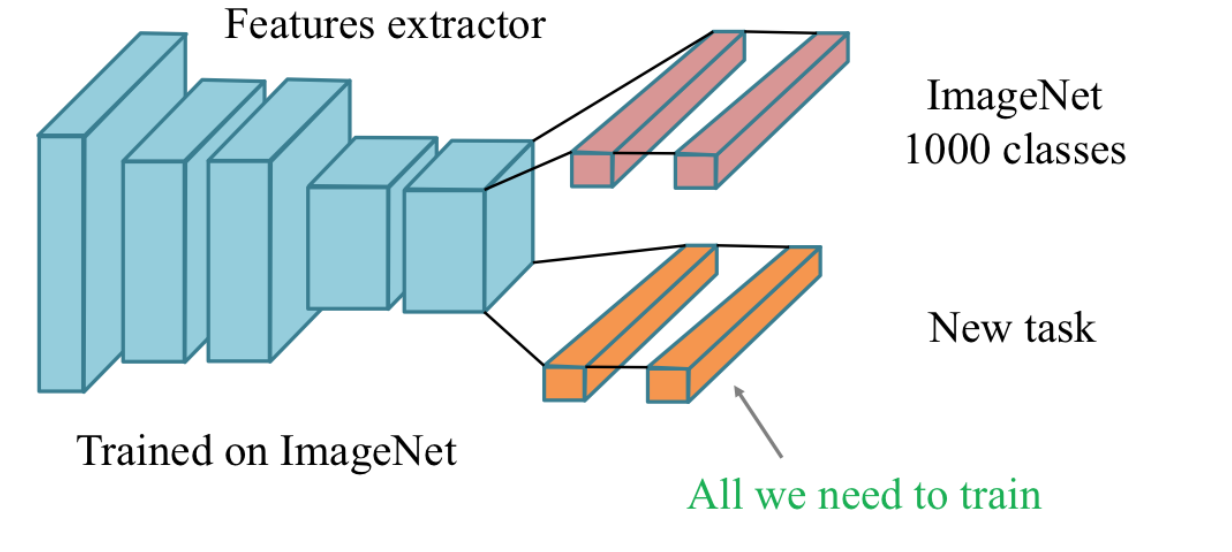
\includegraphics[width=.8\linewidth]{transfer_learning2.png}
\end{center}
\end{frame}


\begin{frame}{Transfer learning}
\begin{wideitemize}
	\item  Нужно меньше данных для обучения, так как нас интересуют лишь последние слои
	\item  Это работает если наша задача похожа на ту, для которой обучалась используемая сетка
	\item  Например, если мы хотим распознавать эмоции, в датасете для нашей сетки должны были быть человеческие лица
\end{wideitemize}
\end{frame}


\begin{frame}{Transfer learning}
\begin{center}
	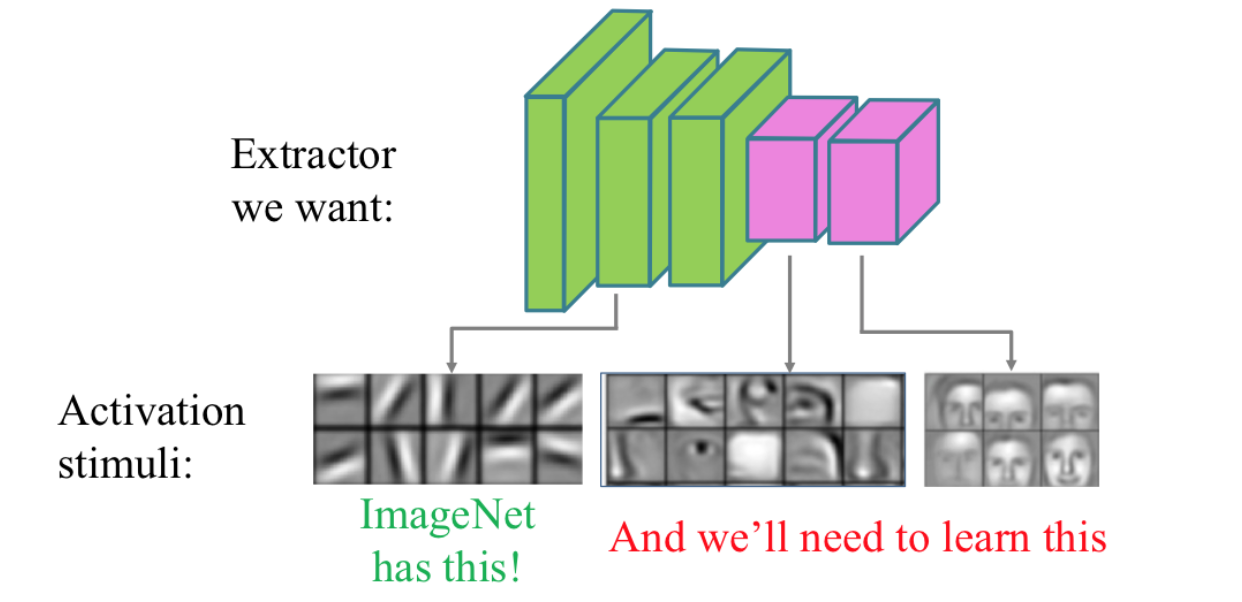
\includegraphics[width=.8\linewidth]{transfer_learning3.png}
\end{center}
\end{frame}


\begin{frame}{Transfer learning}
\begin{center}
	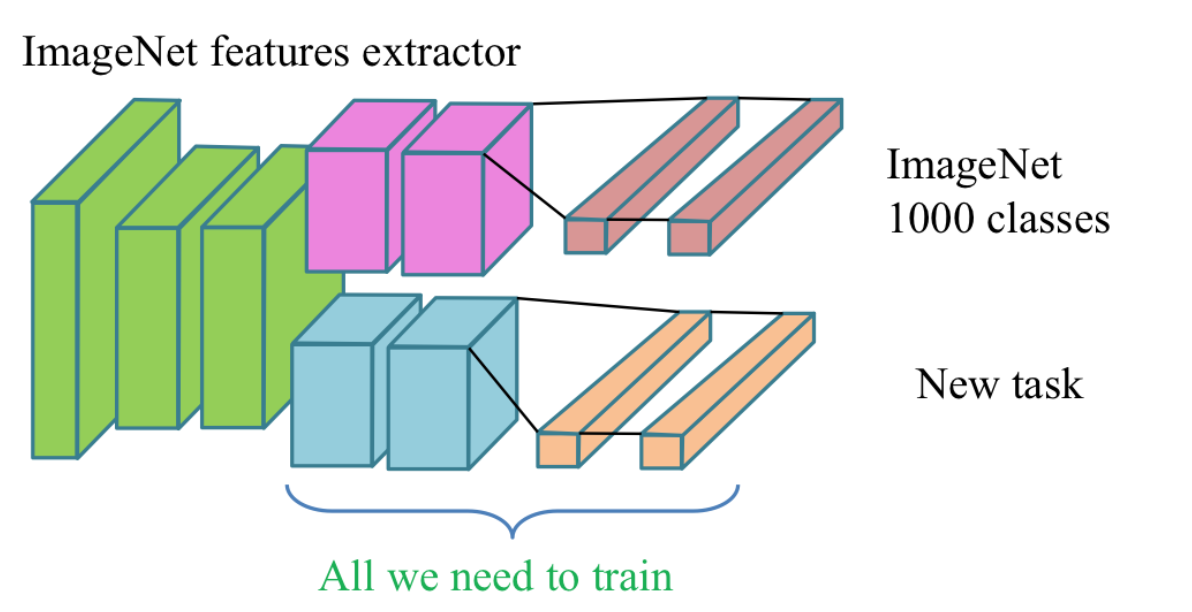
\includegraphics[width=.8\linewidth]{transfer_learning4.png}
\end{center}
\end{frame}

\begin{transitionframe}
	\begin{center}
		\Huge Собираем свой transfer learning!
	\end{center}
\end{transitionframe}

\end{document}
